\documentclass{article}
\usepackage[margin=2cm,bottom=2cm]{geometry}
\usepackage{hyperref}
\usepackage{comment}
\usepackage[utf8]{inputenc}
\usepackage{graphicx}
\usepackage{mathtools}
\usepackage{tikz}
\usepackage{minibox}
\def\checkmark{\tikz\fill[scale=0.4](0,.35) -- (.25,0) -- (1,.7) -- (.25,.15) -- cycle;} 
\graphicspath{ {bootstrapping.png} }

\newcommand\tab[1][1cm]{\hspace*{#1}}

\begin{document}
\title{COMP/CMPE 314 - Principles of Programming Languages - Notes}
\author{Chris Stephenson, Istanbul Bilgi University, Department of Mathematics, and course students}
\maketitle

\section*{WEEK 1}
\section*{Answers of the quiz \#1}
\subsection*{Question \#1}
\subsubsection*{Language}
  \begin{itemize}
        \item A finite alphabet
        \item A set of strings of the symbols in the alphabet (usually infinitive)
   \end{itemize}
 
\subsubsection*{Grammar}
  \begin{itemize}
   \item A set of productions (rewriting rules)
   \item A finite alphabet of terminal symbols
   \item A finite set of non-terminal symbols
   \item A sentence symbol ( S )
  \end{itemize}

Simple language: [a] 
  \begin{itemize}
   \item $S \rightarrow a$
   \item $S \rightarrow aS$ (infinite)
   
   $S \rightarrow number$\newline
   $S \rightarrow S + S$\newline
   $S \rightarrow S * S$\newline
   $S \rightarrow (S)$\newline
   alphabet = [+, *, (), number]
  
  \end{itemize}
  

\subsection*{Question \#2}

  \begin{verbatim}
    (define (interp [a : ArithC]) : number
        (type-case ArithC a
            [numC (n) n]
            [plusC (l r) (+ (numC-n l) (numC-n r))]
            [multC (l r) (* (numC-n l) (numC-n r))]))
  \end{verbatim}
  
  \begin{verbatim}
    In this code;
    (+ 4 3) works but,
    (+ (* 3 7) (+ 4 2)) crashes
  \end{verbatim}
  
  In order to make it work we need to change numC to interp like this

  \begin{verbatim}
    (define (interp [a : ArithC]) : number
        (type-case ArithC a
            [numC (n) n]
            [plusC (l r) (+ (interp l) (interp r))]
            [multC (l r) (* (interp l) (interp r))]))
  \end{verbatim}
  
  
\section*{Programming Languages}
\begin{tabular}{c c}
 \textbf{Programming Languages} & \textbf{Kinds of Programming Languages}\\
 \begin{tabular}{ l c r }
    Java & Assembly & Swift \\
    Python & C & Prolog \\
    Ruby & C\# & Fortran \\
    Objective-C & Racket & R \\
    Lisp & Haskell & Whitespace \\
    Javascript & Pascal & Giuseppe \\
    Scala & HTML & Ada \\
    Pick & Perl & XML \\
    SQL & BASH & XSDL \\
    Scratch &  &  \\
  \end{tabular}
  &
  \begin{tabular}{ c }
    Markup Language \\
    Functional \\
    Object oriented \\
    Procedural \\
    Scripting \\
    Graphical \\
    Experimental \\
    Declarative \\
    Machine \\
  \end{tabular}
\end{tabular}


\begin{flushleft}
The code below is valid in Java and also valid in C. \\
What value does the function/method \verb|funny2| returns?

\begin{verbatim}
 int funny(int a, int b){
    return a + 2 * b;
 }
 
 int funny2(){
    int a = 2;
    return funny(a++, a++);
 }
\end{verbatim}

In this example the value returned in Java and C are different. Java returns 8 but C returns 7.\\
This situation caused by the compilers of this languages. In \verb|funny(a++, a++)| statement Java starts from left \verb|a++| but C starts from right \verb|a++|.\linebreak

Let us consider this now\\
1000000 + 2000000\\
"1000000" + "2000000"\\
In the first example Java returns a negative integer value. Because it assigns numbers default by int and maximum int value is 2,147,483,647.\\
In the second one Java concatenates the two strings like "10000002000000" (But some languages adds them)\linebreak

All programming languages are data formats for data input to other programs.\\
\begin{figure}[h]
   \centering
   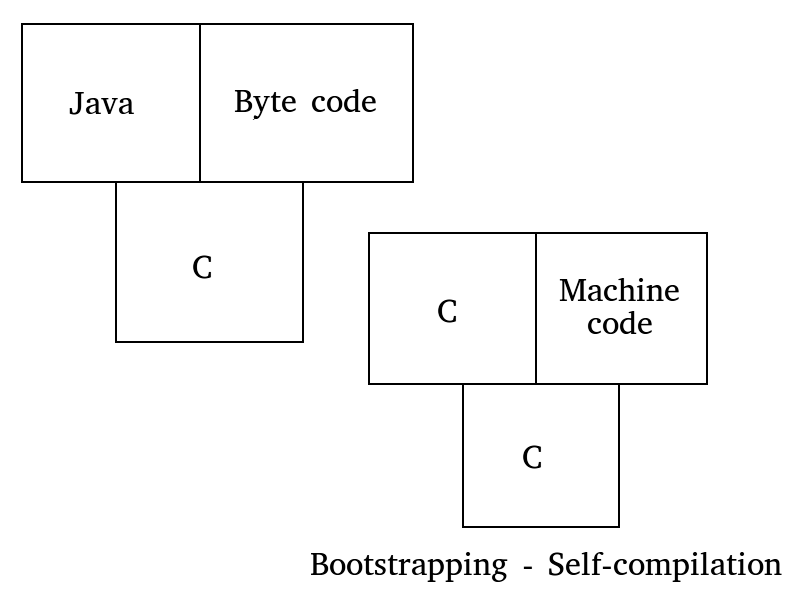
\includegraphics[scale=.2]{bootstrapping.png}
   \caption{Bootstrapping - self compilation}
  \end{figure}
\center{Program text $\xrightarrow{parse}$ Data Structure $\xrightarrow{interp/eval}$ Answer}\\
\begin{verbatim}
 (eval (parse '(+ 2 (* 3 4))))
\end{verbatim}
Parsing is common to all compilers/interpreters
\end{flushleft}
\pagebreak
\section*{WEEK 2}
\section*{Functions/Methods}
\begin{flushleft}
Robert's on Methods;
\begin{itemize}
 \item "Hiding complexity"
 \item "Tools for programmers"
 \item "Method calls as expressions"
 \item "Method calls as messages"
\end{itemize}
"The calling mechanism is that the actual parameters are copied to the formal parameters and the code is executed."\\
\emph{it's a lie!}\\
\bigskip
\section*{How methods are used?}
\tab{Within a function/method you can call another method (We have certainly done that! Example: \verb|Math.min()|)}\\
{Missing:} You can call a method in the expression for the actual parameters;\\
\end{flushleft}
\center{\verb|myMethod(Math.max(a, b));| $\leftarrow$ Piping methods}\\
\begin{flushleft}
$\star$ Linking codes is very powerful.\\
\bigskip
\begin{itemize}
 \item Used for decomposition - Break a problem into pieces
 \item Used for algorithms - Abstraction\\
 (Example: Binary search)\\
\end{itemize}
\end{flushleft}
\begin{flushleft}
\centerline{\noindent\rule{18cm}{0.4pt}}
\tab{In the below java code which is taken from "The Art and Science of java" lets calculate the following equation:}\\
\center{$\binom{n}{r} = \frac{n!}{(n-r)! r!}$}\\
\begin{verbatim}
private int factorial(int n) {
  int result = 1;
  for (int i = 1; i <= n; i++) {
    result *= i;
  }
  return result;
}

public int combinations(int n, int k) {
  return factorial(n) / (factorial(k) * factorial(n - k));
}
\end{verbatim}
\end{flushleft}

\begin{flushleft}
\tab{If we try to calculate \verb|combinations(15, 2)| java will return \verb|-4| which is incorrect and there is no error information. It should return 105. This is because of the max integer limits.}\\
\bigskip
The calculation should be done like this;
\begin{verbatim}
public int computeBinomialCoefficient(int n, int k) {
  int ans = 1;
  k = Math.min(k, n - k);
  for (int i = 0; i < k; i++) {
    ans = ans * (n - k + 1 + i);
    ans = ans / (i + 1);
  }
  return ans;
}
\end{verbatim}
\centerline{\noindent\rule{18cm}{0.4pt}}
\tab{We wrote \underline{a calculator} to make a programming language, we need to add \underline{abstraction}. (= generalisation. In place of numbers we will use \underline{identifiers} in our calculations.)}\\
Example: 
\begin{verbatim}
 int square(int x){ // Here x is formal parameter and bound identifier
  return x * x;
 }
\end{verbatim}
$\vdots$\\
\underline{application}
\begin{verbatim}
 println(" " + square(7)); // Here "7" is the actual parameter
\end{verbatim}
\tab{We evaluate the body of the function by substituting the \underline{actual} parameter for the formal parameter in the body of the function.}\\
\tab{We need to extend our data definition.}\\
\tab{We need to add;}\\
\begin{itemize}
 \item Function definition
 \item Function application
\end{itemize}
\tab{To start with we will keep our function definitions seperate.}\\
\tab{Our functions will have a seperate \underline{namespace}.}\\
\tab{Our interpreter will have two inputs - a list of function definitions - as an expression.}\\
(Which may include function applications)



\section*{What does a function have?}
\begin{flushleft}
\begin{itemize}
 \item A formal parameter - name (identifier)
 \item A body - expression (in our extended version)
 \item A name - identifier (in the function name namespace)
 \item Function name - identifier in the function name namespace
 \item Actual parameter - identifier
\end{itemize}
\tab{Extend our expression data definition.}\\
\tab{We need to add two more variants.}\\
\begin{itemize}
 \item Function application
 \item Identifier
\end{itemize}
\tab{We need to extend the interpreter to deal with the two new variants in the data definition.}
\begin{itemize}
 \item Identifier $\rightarrow$ error
 \item Function application\\
 \verb|(apply (find-function function-list function-name) actual-parameter)|
\end{itemize}
\tab{Statement of purpose for apply, substitute the actual parameter for the formal parameter everywhere in the body of the function, then evaluate the result.}

\begin{verbatim}
 (define '(apply function-definition actual-parameter){
  (interp (subst (function-definition formal-parameter) actual-parameters))
 })
\end{verbatim}
\textbf{What does subst do?}\\
name expression expression $\rightarrow$ expression

\underline{Template:}\\
number $\rightarrow$ number\\
arith-expression $\rightarrow$ same expression but subst the operands\\
identifier $\rightarrow$ if the identifier is the identifier to be substitued, we replace it\\
function application $\rightarrow$ function application, but subst the actual parameter\\
\bigskip
\textbf{The syntax of the $\lambda$-calculus:}\\
$\Lambda \rightarrow \vartheta$ \\
$\Lambda \rightarrow$ ($\lambda \vartheta \lambda$)\\
$\Lambda \rightarrow$ ($\Lambda \Lambda$)\\
\textbf{Valid sentences:}\\
$\mathit{a}$\\
($\mathit{a}$ $\mathit{b}$)\\
($\lambda$ $\mathit{x}$ $\mathit{x}$) - informally this is the identity function\\
($\mathit{a}$ $\mathit{b}$ $\mathit{c}$) - \textit{not valid}\\
($\lambda$ $\mathit{f}$ ($\lambda$ $\mathit{x}$ ($\mathit{f}$ ($\mathit{f}$ $\mathit{x}$)))) - a function doubler\\
($\lambda$ $\mathit{v}$ ($\mathit{...}$))
\end{flushleft}
\pagebreak

\section*{WEEK 3}
\section*{A program that looks the same but evaluates to two different answers should worry us!}
\begin{flushleft}
The following function/method is both works on Java and C, but when we compile it gives different results.
\begin{verbatim}
 int funny (int a, int b){
   return a * 2 + b;
 }

 int haha () {
   int z = 2;
   return funny (z++, z++);
}
\end{verbatim}
This method/function is legit for both languages.\\
\bigskip
In C, we can compile it with one easy step. For this, we need to add C header files and main function.
\begin{verbatim}
#include<stdio.h>

int funny (int a, int b){
  return a * 2 + b;
}

int haha () {
  int z = 2;
  return funny (z++, z++);
}

int main(int argc, char** argv) {
  printf("\n\nThe answer in C is %d\n\n", haha());
  return 0;
}
\end{verbatim}
The output of the program is:\\
\verb|The answer in C is 8|\\
\bigskip
In Java we need to change the methods a little bit. We should add static at the beginning of the methods in order to compile.\\
We can do this without changing the main file via terminal.\\
\begin{verbatim}
 cat funnypre.java | cat - funnyhaha | sed -e 's/^int/static int/g' | cat - funnypost.java
\end{verbatim}
(The files are in the course github repository.)\\
\pagebreak
Output of the code is:
\begin{verbatim}
class Funny{

static int funny (int a, int b){
  return a * 2 + b;
}

static int haha () {
  int z = 2;
  return funny (z++, z++);
} 

public static void main(String[] args){
  System.out.println("\n\nThe answer in Java is " + haha() + "\n\n");
}

}
\end{verbatim}
The output of the program is:\\
\verb|The answer in Java is 7|\\
\bigskip
We can write and compile codes without using Eclipse.\\
Integrated Development Environment (IDE) $ \rightarrow $ Eclipse\\
Unintegrated Development Environment $ \rightarrow $ Terminal\\
\bigskip
For repetitive jobs we should write bash scripts.\\
Example for C:
\begin{verbatim}
cat funnypre.c funnyhaha funnypost.c > funny.c
gcc funny.c -o funny
./funny
\end{verbatim}

\centerline{\noindent\rule{18cm}{0.4pt}}
\bigskip
\textbf{z++}\\
\bigskip
The \verb|++| post operator produces a value the same as the value of its operand. But it changes the subsequent value of the operand as a \underline{side effect.}\\ 
In a program using a for loop to process an array we have (maybe) unnecessary state.\\
Look at Hadoop - Map reduce $ \leftarrow $ must be stateless (big data)\\
\bigskip
\centerline{text $\xrightarrow{parse}$ first representation $\xrightarrow{desugar}$ second representation $\xrightarrow{eval}$ evaluation}
\centerline{"desugaring" = "macro processing"}
\bigskip
For example in Racket, cond is desugared into a series of nested if statements.\\
\bigskip
What does our program evaluation look like?
\begin{verbatim}
 (eval (desugar (parse '(* (-3) (+ 7 8)))))
\end{verbatim}

\centerline{\noindent\rule{18cm}{0.4pt}}
\pagebreak
\textbf{Rules:}\\
$\lambda \rightarrow \mathit{v}$  identifier\\
$\lambda \rightarrow ( \lambda \mathit{v} \Lambda )$ anonymous function definition\\
$\lambda \rightarrow ( \Lambda \Lambda )$ function application \\

\bigskip
$( \mathit{a} $ $ ( \mathit{b}$ $ \mathit{c} ))$ \checkmark\\
$\mathit{a}$ \checkmark\\
$(\mathit{a})$ x \\
$(\mathit{a}$ $\mathit{b})$ \checkmark\\

\centerline{\noindent\rule{18cm}{0.4pt}}
\bigskip
$(\lambda$ $\mathit{x}$ $\mathit{x}) \rightarrow$ identity function$$$$
\begin{verbatim}
int funny(int y){
  return y;
}
\end{verbatim}
$((\lambda$ $\mathit{x}$ $\mathit{x})$ $(\mathit{a}$ $\mathit{b}))$\\
In here x is bound, a and b are free\\
\bigskip
A "complete" program will have no "free" identifiers.\\
A part of that program may have free identifiers.\\

\begin{itemize}
 \item If $\mathit{M}$ is an identifier, $\mathit{x}$. $\mathit{FI(M) = {X}}$
 \item If $\mathit{M}$ is an application $(\mathit{M1}$ $ \mathit{M2})$. $\mathit{FI(M) = FI(M1) \cup FI(M2)}$
 \item If $\mathit{M}$ is a definition $(\lambda$ $\mathit{x}$ $\mathit{M1})$. $\mathit{FI(M1) - }$ \{$\mathit{x}$\}
\end{itemize} 
\bigskip
$\mathit{FI[(\lambda x \space{} (\lambda \space{} y \space{} x ))] = \{\}}$\\
$\mathit{FI[(\lambda y x)] = \{x\}}$
\centerline{\noindent\rule{18cm}{0.4pt}}
\bigskip
\textbf{If statement}\\
True:\\
$\mathit{T = (\lambda x (\lambda y x))}$\\
$\mathit{(T \space{} a) \xrightarrow{\beta} (\lambda \space{} y \space{} a)}$\\
$\mathit{((T \space{} a) \space{} b) \xrightarrow{\beta} a}$\\
\bigskip
False:\\
$\mathit{F = (\lambda \space{} x \space{} (\lambda \space{} y \space{} y))}$\\
$\mathit{((F a) b) \xrightarrow{\beta} b}$
\end{flushleft}
\end{flushleft}
\pagebreak
\begin{flushleft}
\section*{WEEK 4}
\section*{Lies and Equality (In Java and Other Languages)}
\end{flushleft}
\begin{flushleft}
In Java;
\begin{itemize}
 \item "\verb|=|" does not mean "equals" (its assignment)
 \item "\verb|&|" does not mean "and" (its bitwise and)
 \item "|" does not mean "or" (its bitwise or)
 \item "\verb|!|" does not mean "surprise"
 \item "\verb|int|" does not mean "integer"
 \item "\verb|Integer|" does not mean "integer"
 \item "\verb|BigInteger|" does not mean "BigInteger"
\end{itemize}
\bigskip
\begin{itemize}
 \item We use "\verb|==|" for "equals"
 \item We use "\verb|&&|" for "logical and"
 \item We use "||" for "logical or"
\end{itemize}
\begin{flushleft}
 This things are left from C which was invented as high level assembler, not high level language.\\
 \verb|int| \underline{means} a 32 bit two's complement quantity (now most compilers are 64 bit)
\end{flushleft}
\bigskip
\begin{flushleft}
 If I declare \verb|MyClass a;|\\
 \verb|a| is not necessarily an object of class \verb|MyClass|.
\end{flushleft}
\bigskip
\section*{Equality}
\subsection*{What does == mean?}
\begin{verbatim}
class Equality {

  public static void main (String[] args) {
    MyInteger a = new MyInteger(42);
    MyInteger b = new MyInteger(42);
    MyInteger c = new MyInteger(43);
    MyInteger d = c;
    String s1 = "Chris";
    String s2 = "Chris";
    System.out.println("\n a = " + a + ",b = " + b + "\n");
    System.out.println("\n a == b is " + (a == b) + "\n");
    System.out.println("\n s1 == s2 is " + (s1 == s2) + "\n");
    System.out.println("\nd = " + d + "\n");
    System.out.println("\n c == d is " + (c == d) + "\n");
    c.setV(44);
    System.out.println("\n c = " + c +  "\n");
  }
}
\end{verbatim}
\bigskip
\begin{verbatim}
class MyInteger {
  int value;
  
  MyInteger (int v) {
    value = v;
  }

  public String toString () {
    return "" + value;
  }

  public void setV (int v) {
    value = v;
  }
}
\end{verbatim}
\bigskip
Output:
\begin{verbatim}
 a = 42,b = 42


 a == b is false


 s1 == s2 is true


d = 43


 c == d is true


 c = 44
\end{verbatim}

\begin{flushleft}
 It does \underline{not} mean "equal in value" (necessarity)\\
 \verb|setV| method makes our program mutable.\\
 Java is broken. \verb|NullPointerException| is most likely seen error and it causes programs to crash.\\
 The best way to solve this problem is to make our programs \textbf{immutable}.
\end{flushleft}
\begin{verbatim}
 String a = "Chris";
 String b = "Chris";
\end{verbatim}
\begin{flushleft}
 In Java Strings are immutable!
\end{flushleft}
\url{http://javapractices.com}\\
\bigskip
\centerline{\noindent\rule{18cm}{0.4pt}}
\bigskip
\begin{flushleft}
 Our program;\\
 \begin{verbatim}
  '(((fundef factorial n (if2 n 1 (* n (factorial (- n 1))))) (factorial 3))
 \end{verbatim}
 parse + desugar
 \begin{verbatim}
  (appC 'factorial (numC 3))
 
  (ifzC (idC 'n) (numc 1) (mulC (idC 'n) (appC 'factorial (subC (idC 'n) (numC1)))
  
  (idC 'n)'s will be changed with (numC 3)
 \end{verbatim}
 \end{flushleft}
\bigskip
\centerline{\noindent\rule{18cm}{0.4pt}}
\section*{$\alpha$ Transformation}
($\lambda$ $\mathit{x}$ $\mathit{M}$) $\equiv$ ($\lambda$ $\mathit{y}$ $\mathit{M}$ $\mathit{[}$ $\mathit{x}$:=$\mathit{y}$ $\mathit{]}$)

\section*{$\eta$ Transformation (Optional)}
($\lambda$ $\mathit{x}$ ($\mathit{f}$ $\mathit{x}$)) $\xrightarrow{\eta}$ $\mathit{f}$

\section*{$\beta$ Transformation}
(($\lambda$ $\mathit{x}$ $\mathit{M}$) $\mathit{N}$) $\xrightarrow{\beta}$ $\mathit{M}$ $\mathit{[}$ $\mathit{x}$ := $\mathit{N}$ $\mathit{]}$
\end{flushleft}
\begin{flushleft}
\bigskip
\section*{WEEK 5}
\section*{The "real" world}
\begin{flushleft}
\textbf{"Evaluation \underline{Strategies}"}\\
\begin{itemize}
 \item a strange word to use?
 \item we make the languages.
\end{itemize}
The problem is that most languages have design defects, so evaluating them is confusing.\\
\bigskip
\textbf{What do we do?}\\
When and What and How parameters are evaluated?
\end{flushleft}

\subsection*{When?}
In Java;
\begin{verbatim}
  myfunc(a, g(b), c + d);
  myFunc(a++, a++, a++);	// order matters!
\end{verbatim}
** Java compiler (javac) starts evaluating from \underline{left} however C compiler (gcc) starts from \underline{right}.**\\
\bigskip

\textbf{Are the parameters evaluated left to right or right to left?}\\
In Java, left to right\\
In C, \underline{UNDEFINED!}? (Different compilers different answers)


\begin{flushleft}
\textbf{\underline{OR}} We cannot evaluate the parameters at all. And simply pass the expressions to the function body. (All programming languages do this for \underline{some} things)\\
Racket is a \underline{strict} language, which means parameters \underline{are} evaluated.
\end{flushleft}

\begin{verbatim}
;#lang lazy
#lang racket
(define (my-if condition t f)
  (cond
    (condition t)
    (else f)))
    
(define (fac n)
  (my-if (< n 1) 1 (* n (fac (- n 1)))))
\end{verbatim}
Here \verb|my-if| looks like a function. But it isn't a function in racket. It tries to calculate parameters first. Thus it leads to infinitive loop.\\
If we uncomment \verb|#lang lazy| it will work. 

\begin{flushleft}
\underline{Except} for \underline{if}\\
In Java \verb|f(a) && g(b)| is a boolean expression\\
They call it "Short circuited evaluation"\\
Evaluated left to right and stop when we know the answer.
\end{flushleft}

\begin{flushleft}
 
\underline{A practical example:}
\begin{verbatim}
  int i = 0;
  while(i < a.length && a[i] != 0) {
    ...
    i++;
  }
  
  while(a[i]!=0 && i<a.length){	// after a swap, what goes wrong?
    ...
    i++;
  }
\end{verbatim}
If the condition goes to \verb|i > a.length|, the \verb|a[i]| throws an error. So the order is important!
\end{flushleft}

\begin{flushleft}
Is evaluation in this language "Strict?" "Non Strict?" "Sometimes Strict?"\\
A different way of binding formal parameters: \noindent\rule{3cm}{0.4pt}
\end{flushleft}
\begin{center}
\textbf{\underline{Environments}}
\end{center}

\begin{flushleft}
\begin{itemize}
 \item Substitution is not how the real world works (For reasons of efficiency)
 \item An environment is an ordered store of identifier/value pairs
 \item For function application we add formal parameter/actual parameter value pairs to the environment and use that environment to evaluate the function body.
 \item Our \underline{evaluator} takes the environment as an additional parameter when the evaluator evaluates an identifier, it looks up the value in the environment.
\end{itemize}

\end{flushleft}
\subsection*{Data Definitions}
An environment is empty \underline{OR} an identifier/value pair plus an environment.
\begin{itemize}
\item look up Env. environment identifier $\rightarrow$ value or \underline{Error}
\item extend Env. environment identifier $\rightarrow$ environment
\end{itemize}
\begin{verbatim}
Example: 
(fundef myFunc (a b c) (+ a (* b c))) //function definition

(myFunc 3 7 (+ 2 9)) //function application
\end{verbatim}

\subsubsection*{Evaluate a function application}
\begin{verbatim}
(eval (extend Env (extend Env (extend Env (empty Env, 'a, 3) 'b, 7) 'c, 11) '(+ a (* b c))))

(fundef f1 x (f2 4))
(fundef f2 y (+ x y))
\end{verbatim}
Whats wrong with f2?\\
It's a free identifier!\\
In Java:
\begin{verbatim}
int f2(int y){
  return x + y;
}
\end{verbatim}
evaluate (f1 42)\\
 x gets bound to 42\\
 y gets bound to 4\\
 (+ x y) looks up these values in the environment\\
 The answer is 46 \textbf{Wrong!!}\\
\bigskip
Identifier capture!\\
This is called "dynamic scope" and it is a bug.
\bigskip
\begin{flushleft}
\underline{The solution} (for now)\\
When we apply a function, do \underline{not} extend the \underline{current environment} with formal parameter/value bindings. Extend the \underline{empty} environment.
\end{flushleft}

\subsubsection*{Grammar}
\begin{flushleft}
$1)$ $\Lambda\rightarrow\upsilon$

$2)$ $\Lambda\rightarrow(\lambda$ 
$\upsilon$
$\Lambda)$

$3)$ $\Lambda\rightarrow(\Lambda$
$\Lambda)$

Data structure and therefore definitions and programs will reflect this.\\
\bigskip
M[x:=N]\\
\end{flushleft}

\begin{flushleft}
$1)$ M is an identifier\\
\tab{a) M=x $\Rightarrow$ M[x	:=N] is N}\\
\tab{b) M$\neq$x $\Rightarrow$ M[x:=N] is M}\\
\bigskip
$2)$ M is an application (just do the two parts)\\
\bigskip
$3)$ M is a function definition\\
\tab{Case (a) is easy $\lambda$yM1, y=x}\\
\tab{Case (b) is hard $\lambda$yM1, y$\neq$x}\\
\end{flushleft}

\subsubsection*{Church Numerals}
\begin{flushleft}
n $\equiv$ ($\lambda$ f ($\lambda$ x (f (f (f...x)))))\\
$\tab{\tab{\tab{\overline{n f's}}}}$
\end{flushleft}

\begin{flushleft}
ChurchB(n) $\equiv$ (f (ChurchB(n -1)))\\
ChurchB(1) $\equiv$ ($\lambda$ f ($\lambda$ x (f x)))\\
\bigskip
Church(n) = ($\lambda$ f (x x (ChurchB(n))))\\
\end{flushleft}

\begin{flushleft}
TWO=($\lambda$ f ($\lambda$ x (f (f x))))\\
ZERO=($\lambda$ f ($\lambda$ x x))\\
\end{flushleft}
\bigskip
\begin{flushleft}
\textbf{A successor function "SUCC"}\\
SUCC=($\lambda$ n ($\lambda$ f ($\lambda$ x (f ((n f) x))))\\
onSUCC=($\lambda$ n ($\lambda$ f ($\lambda$ x ((n f) (f x))))
\end{flushleft}

\begin{flushleft}
To add m and n;\\
($\lambda$ m ($\lambda$ n ((m succ) n)))
\end{flushleft}
\end{flushleft}
\begin{flushleft}
\bigskip
\section*{WEEK 7}
\section*{Evaluation "Strategies"}
\underline{All about function application} - which is the central concept in programming \textbf{IMHO} an oxymoron
\begin{flushleft}
 We looked at \underline{sequence}. (2 weeks ago)
 \begin{itemize}
  \item Strict vs. non-strict
  \item Eager vs. lazy
  \item Left to right vs. right to left
 \end{itemize}
\underline{What} is passed when we apply a function to actual parameter.\\
Example (in Java)\\
\begin{verbatim}
 {
  a = 2;
  myFunc(a);
 }
 
 void myFunc(int a){
  ...
  a = a + 1;
 }
\end{verbatim}
What is the value of \verb|a|?\\
\verb|System.out.println("a is: " + a);| $\rightarrow$ The answer is 2.
\end{flushleft}
\subsection*{Why?}
\begin{flushleft}
 Because Java/C/C\#/Ruby/Python/C++ are, \underline{call by value}\\
 For simple types, most common programming languages are call by value.\\
 The alternative is \underline{call by preference} (PHP \underline{can} do this)
\end{flushleft}
\section*{But what about complex types?}
\underline{Example:} array, structure, object\\
In Java:
\begin{verbatim}
 {
  ...
  a[k] = 2;
  myFunc(a);
  System.out.println("a[k] is " + a");
 }
 
 
 void myFunc(int[] a){
  ...
  a[l] = a[l] + 1;
  ...
 }
\end{verbatim}
\begin{flushleft}
Call by reference for arrays/Structures/Strings/Objects\\
(Except C - C structures are naturally call by value)\\
Java Strings can be considered call by value. (Because Java Strings are immutable)
\end{flushleft}

\section*{SUPER ACCELERATED CMPE313 (SICP - The Purple Book)}
\begin{flushleft}
 What is a list? A list of numbers x?
 \begin{itemize}
  \item Empty
  \item A pair of a number x and a list of number x.
 \end{itemize}
 \begin{verbatim}
  ;; add-up the numbers in a list
  (define (sum-lon lon)
    (cond
      ((empty? lon) 0)
      (else (+ (first lon) (sum-lon (rest lon))))))
      

  (define (mul-lon lon)
    (cond
      ((empty? lon) 1)
      (else (* (first lon) (mul-lon (rest-lon))))))
      
      
  (define (fold combiner null-value lox)
    (cond
      ((empty? lox) null-value)
      (else (combiner (first lox) (fold combiner null-value (rest lox))))))
 \end{verbatim}
 \textbf{fold} is a powerful \underline{abstraction}.\\
 \bigskip
 I want to evaluate a polynomial.\\
 $ {a}_{0} + {a}_{1}x + {a}_{2}{x}^{2} + {a}_{3}{x}^{3} +....+ {a}_{n}{x}^{n} $ \\
 Data definition a polynomial number $\rightarrow$ number\\
 \bigskip
 Horner's rule;\\
 ${a}_{0} + x({a}_{1} + x({a}_{2} + x({a}_{3}...{a}_{n}))))$\\
 \bigskip
 To evaluate a polynomial\\
 \begin{verbatim}
  (define (eval-poly p x)
    (fold (lambda (l r) (+ l (+ l (* x r)) non-empty p))))
 \end{verbatim}
 map
 \begin{verbatim}
  (define (map f lox) 
    (fold (lambda (l r) (cons (f l) (cons (f l) r)) empty lox)))
 \end{verbatim}
\bigskip
 filter
\begin{verbatim}
 (define (filter p? lox)
    (fold (lambda (l r) (if (p? l) (cons l r) empty lox))))
\end{verbatim}
Suppose I am doing a \underline{map} to add 2 to every item in a list:
\begin{verbatim}
 (define (add2 lon)
    (map (lambda (x) (+ x 2)) lon))
    
 (define (mul 7 lon)
    (map (lambda (x) (* x 7)) lon))
    
 (define (curry f x)
    (lambda (y) (f x y)))
\end{verbatim}
Generalizing:
\begin{verbatim}
 (define (arith-map operator constant)
    (map (curry operator constant) lon))
\end{verbatim}
\end{flushleft}
\section*{The $\lambda$-calculus}
\subsubsection*{Summary:}
\begin{flushleft}
$\Lambda\rightarrow\upsilon$ (identifier) \\ 
$\Lambda\rightarrow(\lambda$ $\upsilon$ $\Lambda)$ (definition) \\
$\Lambda\rightarrow(\Lambda$ $\Lambda)$ (application) \\
\bigskip
\underline{$\alpha$ rewriting rule:}\\
($\lambda$ $\upsilon$ $\Lambda$) $\equiv$ ($\lambda$ $\mathit{u}$ $\Lambda$[$\upsilon$:=$\mathit{u}$]) (plagiarizing student rule)\\
\bigskip
\underline{$\eta$ rule (optional):}\\
($\lambda$ $\upsilon$ (f $\upsilon$)) $\equiv$ f\\
\bigskip
\underline{$\beta$ rule:}\\
(($\lambda$ $\upsilon$ ${\Lambda}_{1}$) ${\Lambda}_{2}$ $\xrightarrow{\beta}$ ${\Lambda}_{1}$ [$\upsilon$:=${\Lambda}_{2}$]\\
\bigskip
defining substitution is more complicated\\
$\Lambda$[$\upsilon$:=${\Lambda}_{0}$] - see the slides \\
\begin{itemize}
 \item[(a)] $\Lambda$ = $\mathit{u}$
 \item[] if $\mathit{u}$ = $\upsilon$ $\rightarrow$ ${\Lambda}_{0}$ 
 \item[] else $\Lambda$
 \item[(b)] $\Lambda$ = (${\Lambda}_{1}$ ${\Lambda}_{2}$)
 \item[] (${\Lambda}_{1}$[$\upsilon$=${\Lambda}_{0}$] ${\Lambda}_{2}$[$\upsilon$=${\Lambda}_{0}$]
 \item[(c)] $\Lambda$ = ($\lambda$ $\mathit{u}$ ${\Lambda}_{1}$)
 \subitem$\mathit{(i)}$ $\mathit{u}$ = $\upsilon$ $\rightarrow$ $\Lambda$
 \subitem$\mathit{(ii)}$ $\mathit{u}$ $\neq\upsilon$ $\rightarrow$ if necessary re-letter before substituting in the body.
\end{itemize}
\end{flushleft}
\pagebreak
\section*{Church Numerals}
\begin{flushleft} 
 0 $\equiv$ ($\lambda$ $\mathit{f}$ ($\lambda$ $\mathit{x}$ $\mathit{x}$))\\
 1 $\equiv$ ($\lambda$ $\mathit{f}$ ($\lambda$ $\mathit{x}$ ($\mathit{f}$ $\mathit{x}$)))\\
 2 $\equiv$ ($\lambda$ $\mathit{f}$ ($\lambda$ $\mathit{x}$ ($\mathit{f}$ ($\mathit{f}$ $\mathit{x}$))))\\
\bigskip
\textbf{Successor:}\\
SUCC=($\lambda$ n ($\lambda$  $\mathit{f}$  ($\lambda$  $\mathit{x}$  ( $\mathit{f}$  ((n  $\mathit{f}$ )  $\mathit{x}$ ))))\\
onSUCC=($\lambda$ n ($\lambda$  $\mathit{f}$  ($\lambda$  $\mathit{x}$  ((n  $\mathit{f}$ ) ( $\mathit{f}$   $\mathit{x}$ ))))\\
\bigskip
(($\lambda$ n ($\lambda$  $\mathit{f}$  ($\lambda$  $\mathit{x}$  ( $\mathit{f}$  ((n  $\mathit{f}$ )  $\mathit{x}$ ))))) $\lambda$  $\mathit{f}$  ($\lambda$  $\mathit{x}$  ( $\mathit{f}$   $\mathit{x}$ ))))\\
\bigskip
$\downarrow \beta$\\
\bigskip
($\lambda$  $\mathit{f}$  ($\lambda$  $\mathit{x}$  ( $\mathit{f}$  (($\lambda$  $\mathit{f}$  ($\lambda$  $\mathit{x}$  ( $\mathit{f}$   $\mathit{x}$ )))  $\mathit{f}$ )  $\mathit{x}$ ))))\\
\bigskip
$\downarrow \beta$\\
\bigskip
($\lambda$  $\mathit{f}$  ($\lambda$  $\mathit{x}$  ( $\mathit{f}$  (($\lambda$  $\mathit{x}$  ( $\mathit{f}$   $\mathit{x}$ )))  $\mathit{x}$ ))))\\
\bigskip
$\downarrow \beta$\\
\bigskip
($\lambda$  $\mathit{f}$  ($\lambda$  $\mathit{x}$  ( $\mathit{f}$  ( $\mathit{f}$   $\mathit{x}$ )))) $\equiv$ 2!
\end{flushleft}
\end{flushleft}
\bigskip
\begin{flushleft}
 \section*{WEEK 8}
 \section*{Haskell}
\begin{itemize}
 \item Purely functional - no state of programs
 \item Statically typed
 \item Lazy
\end{itemize}

\section*{Functional Programming}
\begin{itemize}
 \item Functions are first class values.
 \item No state / no side effects
\end{itemize}
\begin{flushleft}
 How can we do this in our interpreter?\\
 A function application \verb|(name expr)| will no longer be.\\
 It will be \verb|(expr expr)|\\
 This means we have more than one \underline{type} of expression. So runtime types. So we can have booleans.
\end{flushleft}
\section{Types}
\section{How will functions be named?}
\begin{flushleft}
\begin{itemize}
 \item Just like any other expression.
 \item Identifiers (which are always formal parameters) and are then applied to actual parameters.
 \item This will also be true for functions.
\end{itemize}
\bigskip
What would we like to have?\\
\begin{verbatim}
 (let
    (myfunc (lambda (x) (+ x 3)))      function definition
    (myfunc2 (lambda (y) (* y 4)))     function definition
    ...<program>                       expressions
    )
\end{verbatim}
\underline{let} is \underline{sugar}.\\
Desugaring the let;
\begin{verbatim}
 ((lambda (myfunc myfunc2)
    <program>)
    (lambda (x) (+ x 3)) (lambda (y) (* y 4)))
\end{verbatim}
\underline{Example:}
\begin{verbatim}
 (let
      ((double (lambda (x) (* x 2)))
    (double 7))
 
 ((lambda (double)
    (double 7))
      (lambda (x) (* x 2)))
\end{verbatim}
\begin{verbatim}
 (let
    ((multiply-list-by-n (lambda (l n) (map (lambda ((x) (* x n)) l))
      (multiply-list-by-n '(4 5) 3)
      (multiply-list-by-n '(5 6) 7)))))
\end{verbatim}
\end{flushleft}

\section{Closure}
\begin{flushleft}
 We need to distinguish function definitions from \underline{function values} when we \underline{evaluate} a function definition we get a \underline{function value}.\\
 \bigskip
 function definition $\xrightarrow{one->many}$ function value\\
 \bigskip
 A \underline{function value} is a function definition \underline{plus} the environment at the point where the function value was evaluated. This is called \underline{closure}.
\end{flushleft}

\section{When we apply a function value?}
\begin{flushleft}
 Extend the environment in the function value with the bindings of the formal parameters to the actual parameters.
\end{flushleft}
\subsection{Sugaring the $\lambda$-calculus}
\begin{flushleft}
 \underline{Some definitions}\\
 ($F^{0}$M)  $\equiv$ M\\
 ($F^{n+1}$M)  $\equiv$ F($F^{n}$M))\\
 \bigskip
 $C_n$ = Church numeral $\mathit{n}$\\
 \bigskip
 So,\\
 $C_n$ $\equiv$($\lambda$ $\mathit{f}$ ($\lambda$  $\mathit{x}$  ( $f^{n}$  $\mathit{x}$)))\\
 $C_0$ $\equiv$($\lambda$ $\mathit{f}$ ($\lambda$  $\mathit{x}$  ( $f^{0}$  $\mathit{x}$)))  $\equiv$ ($\lambda$ $\mathit{f}$ ($\lambda$  $\mathit{x}$   $\mathit{x}$))\\
 $C_1$ $\equiv$($\lambda$ $\mathit{f}$ ($\lambda$  $\mathit{x}$  ($f^{1}$  $\mathit{x}$)))  $\equiv$ ($\lambda$ $\mathit{f}$ ($\lambda$  $\mathit{x}$  ($\mathit{f}$  $\mathit{x}$)))\\
 $C_2$ $\equiv$($\lambda$ $\mathit{f}$ ($\lambda$  $\mathit{x}$  ($f^{2}$  $\mathit{x}$)))  $\equiv$ ($\lambda$ $\mathit{f}$ ($\lambda$  $\mathit{x}$  ($\mathit{f}$ ($\mathit{f}$  $\mathit{x}$))))\\
 \bigskip
 \underline{LET} - as we did for our interpreter\\
 \begin{tabular}{l l}
  SUCC & ($\lambda$ $\mathit{n}$ ($\lambda$ $\mathit{f}$ ( $\lambda$ $\mathit{x}$) ($\mathit{f}$ (($\mathit{n}$ $\mathit{f}$) $\mathit{x}$))))\\
  TRUE & ($\lambda$ $\mathit{x}$ ($\lambda$ $\mathit{y}$ $\mathit{x}$))\\
  FALSE & ($\lambda$ $\mathit{x}$ ($\lambda$ $\mathit{y}$ $\mathit{y}$))\\
  IF & ($\lambda$ $\mathit{a}$ ($\lambda$ $\mathit{b}$ ($\lambda$ $\mathit{c}$ (($\mathit{a}$ $\mathit{b}$) $\mathit{c}$))))\\
  ZERO? & ($\lambda$ $\mathit{n}$ (($\mathit{n}$ ($\lambda$ $\mathit{x}$ $\mathit{FALSE}$)) $\mathit{TRUE}$))\\
 \end{tabular}
 \end{flushleft}
 \subsection{Data Structures}
 If we can make a pair, we can make a data structure.\\
 What are the semantics of \verb|CONS FIRST REST| (in Racket)?\\
 \begin{itemize}
  \item[] \verb|(FIRST (CONS A B)) = A        -> necessary semantics|
  \item[] \verb|(REST (CONS A B)) = B         -> necessary semantics|
 \end{itemize}
 \bigskip
\begin{tabular}{l l}
 CONS & ($\lambda$ $\mathit{a}$ ($\lambda$ $\mathit{b}$ ($\lambda$ $\mathit{f}$ (($\mathit{f}$ $\mathit{a}$) $\mathit{b}$))))\\
 FIRST & ($\lambda$ $\mathit{c}$ ($\mathit{c}$ $\mathit{TRUE}$))\\
 REST & ($\lambda$ $\mathit{c}$ ($\mathit{c}$ $\mathit{FALSE}$))\\
\end{tabular}
\end{flushleft}
\bigskip
\begin{flushleft}
 \section*{WEEK 9}
 \section*{Laziness in Racket}
\begin{flushleft}
\underline{CONS} - We want it to be lazy\\
How can we get laziness in an eager language?\\
\begin{verbatim}
 (lambda () <expr>) --> promise
\end{verbatim}
to force our promise to evaluate we just write \verb|(promise)|\\
\begin{verbatim}
 (delay (+ 2 3))
\end{verbatim}
\verb|define-syntax-rule| makes a function that operates on program text. It's a way of providing syntactic sugar. 
\end{flushleft}

\section*{Hamming Code}
\begin{flushleft}
 \underline{Hamming's Problem}\\
 Produce a list of numbers only divisible by the prime numbers 3, 5, 7 and no other prime number in order 1 3 5 7 9 15 21 25 27 35
\end{flushleft}

\section*{Georg Contor}
\begin{flushleft}
The hotel with an infinite number of rooms is full.\\
\bigskip
\begin{tabular}{c | c c c c}
  - & 1 & 2 & 3 & 4 \\
  \hline
  0 & / & / & / & / \\
  1 & / & / & / &  \\
  2 & / & / &  &  \\
  3 & / &  &  &  \\
\end{tabular}
\bigskip
\\What is our interpreter now going to look like?\\
We have \underline{function values}. So we need a different way of naming functions.\\
The only way we now have of creating names is as function parameters.\\
This is cumbersome to write in the target language.\\
Why don't we use the syntactic sugar of a Racket style let statement?
\pagebreak
\begin{verbatim}
 (let
    <def. list>
    expr)
    
 <def. list> --> ((name1 expr1)
                  (name2 expr2)
                  (namen exprn)
                  ...)
                  
 (let <def. list> expr) --> (let ((name1 expr1))
                               (let ((name2 expr2))
                                  (let ...
                                     expr)))
\end{verbatim}
desugar2

\verb|(let (name exp) program)| $ \xrightarrow{desugar} $ \verb|((lambda name program) expr)| \\

\subsection*{Grammar for our target language:}
\begin{itemize}
 \item[] S $\rightarrow$ identifier
 \item[] S $\rightarrow$ (S S)
 \item[] S $\rightarrow$ ($\lambda$ identifier S)
 \item[] S $\rightarrow$ (let (identifier S) S)
 \item[] S $\rightarrow$ number
 \item[] S $\rightarrow$ (+ S S) ...
\end{itemize}
When we want multi-parameter functions we can also do this by desugaring.\\
\bigskip
\verb|(lambda (| $v_1$ $v_2$ $v_3$ \verb|expr)| $\xrightarrow{desugar}$ \verb|(lambda| $v_1$ \verb|(lambda| $v_2$ \verb|(lambda| $v_3$ ... \verb|expr))))|\\
\bigskip
\verb|(a b c d)| $\xrightarrow{desugar}$ \verb|(((a b) c) d)|
\end{flushleft}

\subsection*{$\lambda$-calculus}
\begin{flushleft}
  \begin{itemize}
   \item[] (($\mathit{I}$ $\mathit{M}$) $\mathit{N}$) $\rightarrow$ ($\mathit{M}$ $\mathit{N}$)
   \item[] exponentiation = identity function
  \end{itemize}
The predecessor function is \underline{hard.}\\
\verb|(PRED n)| what we want it \verb|n-1|\\
Think of a pipeline\\
\bigskip
Let us program this transformation on pairs.\\
$\mathit{[} \mathit{a,b} \mathit{]}$  $\rightarrow$ $\mathit{[} \mathit{b, (SUCC}$ B$) \mathit{]}$

\begin{verbatim}
 (lambda n
    (FIRST ((n (lambda c
                  ((CONS (REST c)) (SUCC (REST c))))))
                  ((CONS ZERO) ZERO)))
\end{verbatim}
This is a \verb|PRED| function.\\
\pagebreak
\subsection*{Observation}
\begin{tabular}{l c l}
 ($\lambda$ x x)		& $\equiv$ & ($\lambda$ y y) ($\alpha$ transformation)\\
 ($\lambda$ x ($\lambda$ y y))	& $\equiv$ & ($\lambda$ a ($\lambda$ b b)) ($\alpha$ transformation)\\
 ($\lambda$ x ($\lambda$ y x))	& $\neq$   & ($\lambda$ a ($\lambda$ b b))\\
\end{tabular}
\bigskip
\\What is the normal form?\\
What is the essential difference?\\
\end{flushleft}
\bigskip
\begin{flushleft}
\subsection*{de Bruijn indices}
\begin{tabular}{l c l}
  ($\lambda$ x x)		& $\rightarrow$		& ($\lambda$ 1)\\
  ($\lambda$ ($\lambda$ 1))	& $\rightarrow$		& ($\lambda$ ($\lambda$ 1))\\
  ($\lambda$ ($\lambda$ 2))	& $\rightarrow$		& ($\lambda$ ($\lambda$ 1))\\
\end{tabular}
\end{flushleft}
\end{flushleft}
\bigskip
\begin{flushleft}
 \section*{WEEK 10}
 \section*{HASKELL}
\begin{itemize}
 \item[1] Functional - function values are first class values\\
  no  assignment, no side effects
  \item[2] Lazy - example: all lists can be infinitive. No special treatment is needed for infinitive lists
  \item[3] Sophisticated Type System - That allow generic programming\\
  variable types
  \item[4] Lots of interesting sugar
\end{itemize}
 \begin{flushleft}
 \framebox(150,40){\minibox{Java is not the solution\\ Java is the \underline{problem.}}}
 \end{flushleft}
 
 \section*{$\beta$ Transformations}
 \begin{flushleft}
  Why did we object to identifier capture?\\
  ($\lambda$ $\mathit{m}$ ($\lambda$ $\mathit{n}$ ((($\lambda$ $\mathit{x}$ ($\lambda$ $\mathit{y}$ ($\mathit{x}$ $\mathit{y}$))) $\mathit{m}$) $\mathit{n}$))) $\mathit{y}$) $\mathit{x}$) \\
  ($\lambda$ $\mathit{m}$ ($\lambda$ $\mathit{n}$ ((($\lambda$ $\mathit{x}$ ($\lambda$ $\mathit{y}$ ($\mathit{x}$ $\mathit{y}$))) $\mathit{m}$) $\mathit{n}$))) $\mathit{y}$) $\mathit{x}$) \\
  If we have identifier capture the result of the $\beta$ transformations depends on the order they are done in.\\
  \bigskip
  Is it the case that our definition of $\beta$ transformation (including the substitution rule) avoids the problem?\\
  \bigskip
  \section*{The Curch-Rosser Property aka the "Diamond Property"}
  If a $\lambda$-sentence $\mathit{M}$ can be transformed by chains of $\beta$ transformations into sentences $\mathit{M_1}$ and $\mathit{M_2}$, then there exist (possibly empty) chains of $\beta$ transformations that transform $\mathit{M}$ and $\mathit{M_2}$ into some sentence $\mathit{M_3}$\\
  \bigskip
  \underline{A normal form:} is a $\lambda$ sentence in which no $\beta$ transformation is possible.\\
  If Church-Rosser applies every sentence has \underline{at most one} normal form. \\
  \underline{Proof:} Suppose $\mathit{M}$ has 2 normal forms, $\mathit{M_1}$ and $\mathit{M_2}$. But Church-Rosser tells us that there are chains of $\beta$ transformations that transform $\mathit{M_1}$ $\mathit{M_2}$ into $\mathit{M_3}$. But $\mathit{M_1}$ $\mathit{M_2}$ are normal forms, so these chains must be empty. So $\mathit{M_1}$ =  $\mathit{M_2}$ = $\mathit{M_3}$\\
  \bigskip
  (($\lambda$ $\mathit{x}$ $\mathit{y}$) (($\lambda$ $\mathit{x}$ ($\mathit{x}$ $\mathit{x}$)) ($\lambda$ $\mathit{x}$ ($\mathit{x}$ $\mathit{x}$))))\\
 \end{flushleft}
\end{flushleft}
\begin{flushleft}
 \section*{WEEK 11}
 \begin{flushleft}
 Use map to write Haskell function that multiplies every element of a possibly infinite list of integers by n.\\
 \begin{verbatim}
  mulList :: Integer -> [Integer] -> [Integer]
  mulList n l = map ((*) n) l
 \end{verbatim}
The signature of map?\\
\begin{verbatim}
 map :: (x -> y) -> [x] -> [y]
\end{verbatim}
Type signature of *?
\begin{verbatim}
 Integer -> Integer -> Integer
\end{verbatim}
\end{flushleft}
\section*{Exercise 3.59 in SICP}
\begin{flushleft}
 \underline{Infinite series}\\
 \verb|S = |  $a_0 + a_1x + a_2x^2 + a_3x^3 + ... $\\
 treat an infinite series as an infinite list $[a_0, a_1]$\\
 \bigskip
 Consider $\int_{0}^{x} Sdx$ can we write an \underline{integrate} function?\\
 \bigskip
 Contract \verb|[Number] -> [Number]|\\
 $$\int_{0}^{x} (a_0 + a_1x + a_2x^2 + a_3x^3 + ...) dx = a_0x + \frac{a_1x^2}{2} + \frac{a_2x^3}{3} + ...$$\\
 \begin{verbatim}
  integrate s = 1 : zipWith (/) S [1,2..]
 \end{verbatim}
 \underline{zipWith signature}\\
 \verb|(a -> b -> c) -> [a] -> [b] -> [c]|\\
 \bigskip
 Consider a function such that $\int f(x)dx = f(x)$\\
 \begin{verbatim}
  funny = integrate funny
  
  powers x = 1 : map(* x) (powers x)
 \end{verbatim}
\end{flushleft}
\section*{The most beautiful function}
\begin{flushleft}
 \begin{verbatim}
  (LET ((x (lambda x x)) (succ (lambda n (lambda f (lambda x (f ((n f) x))))))
         <body>)
         
         
  (LETn (v <expr>) <body>)  ==>  ((lambda v <body>) <expr>)
 \end{verbatim}
 we want to write factorial\\
 \begin{verbatim}
  (LET (fac (lambda n (((IF (ZERO ? n)) ONE) (fac (PRED n))))
 \end{verbatim}
 all defined in LETs desugar
 \begin{verbatim}
  ((lambda fac (fac SEVEN)) (lambda n ((IF (ZERO ? N) ONE) (fac (PRED n))))
 \end{verbatim}
 Our factorial function needs to look like this
 \begin{verbatim}
  (lambda fac (lambda n .. fac ..))
 \end{verbatim}
 Then we need to make a closure of fac applied to \underline{itself.}
 \begin{verbatim}
  ((lambda f ((lambda x (f (x x))) (lambda x (f (x x))))) F)
 \end{verbatim}
 $\Big\downarrow{\beta}$\\
 \bigskip
 \verb|((lambda x (F (x x)) (lambda x (F (x x))))| $\equiv$ \verb|(YF)|\\
 \bigskip
 $\Big\downarrow{\beta}$\\
 \bigskip
 \verb|(F ((lambda x (F (x x)) (lambda x (F (x x))))| $\equiv$ \verb|F(YF)|\\
 \bigskip
 \underline{The Y combinator}
\end{flushleft}
\end{flushleft}
\bigskip
\begin{flushleft}
 \section*{WEEK 12}
 \section*{Haskell}
\begin{flushleft}
 \begin{itemize}
  \item has typing
  \item and type interface
 \end{itemize}
 What is the right hand side cosSeries?\\
 It is a list comprehension\\
 \bigskip
 The aim is;\\
 $$1 -\frac{x^2}{2!} + \frac{x^4}{4!} - \frac{x^6}{6!} + ...$$\\
 \begin{verbatim}
  facs = 1 : zipWith (*) facs[2,3,..]
  fibs = 1 : 1 : zipWith (+) fibs (tail fibs)
 \end{verbatim}
\end{flushleft}

\section*{Eratosthenes Sieve}
\begin{flushleft}
 \begin{verbatim}
  isPrime :: [Integer] Integer -> Bool
  isPrime lp n 
           | (head lp) ^ 2 > n = True
           | mod n (head lp) == 0 False
           | otherwise = isPrime(tail lp) n
 
  
  primes = 2 : (filter (isPrime primes) [3,5...])
 \end{verbatim}
\end{flushleft}

\section*{Type Signatures}
\begin{flushleft}
 \begin{verbatim}
  isPrime :: [Integer] -> Integer -> Bool
  
  filter :: (a -> Bool) -> [a] -> [a]
  map :: (a -> b) -> [a] -> [b]
  foldr :: (a-> b -> b) -> b -> [a] -> b
  
  sum = foldr (+) 0
  product = foldr (*) 1
 \end{verbatim}
 Leveraging the Haskell type system - polynomial arithmetic.\\
 $(a_0 + a_1x + a_2x^2 + ... + a_nx^n) \leftarrow$ polynomial in 1 variable.\\
 represent as a list $[a_0, a_1, .. a_n]$\\
 $[a_0, a_1, .. a_n] + [b_0, b_1, .. b_m] = [a_0 + b_0, a_1 + b_1, ..]$\\
 $[a_0, a_1, ..] * [b_0, b_1, .. b_m] = [a_0 * b_0, a_1 * b_0 + a_0 * b_1, .. a_m * b_n]$
\end{flushleft}
\end{flushleft}
\bigskip
\begin{flushleft}
 \section*{WEEK 13}
 \section*{Memory Management}
\begin{flushleft}
 In Java we can allocate memory with \underline{new} keyword.
 \begin{verbatim}
  int[] a = new int[n];
 \end{verbatim}
 In C/C++ we have \underline{malloc} and \underline{free}.\\
 \bigskip
 If we have \underline{manual} memory management;
 \begin{itemize}
  \item[(a)] We can have a memory leak. (forget to free)
  \item[(b)] We can have a catastrophe. (free memory still in use)
 \end{itemize}
 Even this is not cheap.\\
 Especially if we think about \underline{fragmentation}.
 \begin{verbatim}
  +------------------------------------------------+
  |      | free |      | free |      | free |      |
  +------------------------------------------------+
 \end{verbatim}
 Manual is not a good idea. - Leads to problems in practice.\\
 We want an automatic system.\\
 It needs to detect when allocated memory can be handed back.
 \begin{itemize}
  \item We want a system that is \underline{sound}. (does not hand back free memory)
  \item We want a system that is \underline{complete}. (hands back all free memory)
 \end{itemize}
\end{flushleft}

\subsection*{Solution 1 (PHP, Swift)}
\subsubsection*{Reference Counts}
 \begin{flushleft}
  Increase for each new reference to a piece of memory,\\
  decrease when a reference is deleted or overwritten.\\
  When the count drops to \underline{zero} hand back the memory.
  \begin{verbatim}
   class x {
      .. x a = this;    <-- Circular Reference
   }
  \end{verbatim}
  In this example, there is no way to fall zero! It causes memory leak.
 \end{flushleft}

\subsection*{Solution 2 (Java, C\#, Racket, Haskell, ..)}
\subsubsection*{Garbage Collection}
\begin{flushleft}
\begin{itemize}
 \item[] Find the memory in use starting from base references,
 \item[] Mark the memory in use,
 \item[] Free all the rest.
\end{itemize}
\bigskip
\textbf{Cheney (1970)}\\
 \begin{itemize}
  \item[] Divide memory into two,
  \item[] Use A for allocating memory,
  \item[] When A is ``exhausted"
  \item[] Copy referenced memory from A to B
  \item[] Mark the old copies with ''broken hearts"
 \end{itemize}
\bigskip
\textbf{Exploit}\\
\begin{itemize}
 \item Short term allocation
 \item Long term allocation
\end{itemize}
\end{flushleft}

\subsection*{Generational Garbage Collection}
\begin{verbatim}
 (define (substitute [to-sub : lambda] [for : symbol] [in : lambda]) : lambda
      (type-case lambda in
           [lambda-id (id) (if (symbol=? for id) to-sub in)]
           [lambda-apply (lhs rhs) (lambda-apply (substitute to-sub for lhs)
                                                 (substitute to-sub for rhs))]
           [lambda-def (bound body) (if (symbol=? for bound) in
                                    (if (or (not (set-member for (free-identifiers body)))
                                            (not (set-member bound (free-identifiers to-sub)))
                                    (lambda-def bound (substitute to-sub in body)))))]
\end{verbatim}
\end{flushleft}
\bigskip
\begin{flushleft}
 \section*{WEEK 14}
\begin{flushleft}
 \begin{verbatim}
  (LET ((MUL (lambda m (lambda m (lambda f (lambda x (m (n x)))))))) body)
  
  (LET ((id1 bv1) (id2 bv2) ...) <body>)
  
  (LET (id bv) <body>) --> ((lambda id <body>) bv)
  
  (LET (id1 bv1) (LET (id2 bv2) (LET ...) <body>)
 \end{verbatim}
 this is a \underline{fold.}\\
 \pagebreak
 \underline{\textbf{Quiz question answer:}}\\
 \begin{verbatim}
  (LET ((a (b x)) (b c)) (lambda b (c a)))
  
  (LET ((a (b x))) (LET ((b c)) (lambda b (c a))))
  
  ((lambda a ((lambda b (lambda b (c a))) c))) (b x)))
 \end{verbatim}
 \bigskip
 To get a \underline{practical} lambda calculus interpreter we need to always do the \underline{leftmost} $\beta$ transformation.\\
 \underline{Example:} Y combinator will loop if you don't always do the leftmost.\\
 \bigskip
 Consider ($\Lambda_1$ $\Lambda_2$) $\Lambda_1$ is not a def \\
 So we transform $\Lambda_1$ - if after \underline{any} transformation $\Lambda_1$ becomes a def we need to apply it immediately.
\end{flushleft}

\subsection*{Mutation + Sequence}
\begin{flushleft}
 \begin{verbatim}
  a = b;                           c = a;
               not equal to        
  c = a;                           a = b;
 \end{verbatim}
 \underline{Sequence matters!}\\
 \bigskip
 in Racket;\\
 \begin{verbatim}
  (begin
      a1
      a2
      a3
      a4)
 \end{verbatim}
 memory is a \underline{key-value} store\\
 make every value a pair \underline{mem x value}\\
 \verb|(a4 (a3 (a2 (a1 x))))|
 \bigskip
 A general solver for polynomial equations of this form\\
 $a_0 + a_1x + a_2x^2 + ... + a_nx^n = 0$\\
 Present polynomial as array of numbers\\
 $(1 + 2x + 3x^2) (4 + 2x) = 4 + 10x + 16x^2 + 6x^3$\\
 evaluate $a_0 + a_1x + ... + a_nx^n = a_0 + x(a_1 + x(a_2 ... a_n)))))$\\
 $1 + 2x + 3x^2 + 4x^3$  , x=2 $\rightarrow$ 49\\
 Make the polynomial whose roots are $r_0, r_1, r_2, ...$\\
 $(x - r_0) (x - r_1) (x - r_2) ... (x - r_n)$\\
 $(-r_0 + x) (-r_1 + x) (-r_2 + x) ... (-r_n + x)$\\
 $(x - 1) (x - 2) (x - 3) (x - 4)$\\
 $x^4 - 10x^3 + 35x^2 - 50 + 24$\\
 \underline{Need to differentiate a polynomial}\\
 $a_0 + a_1x + a_2x^2 ... $ $\rightarrow$ $a_1 + 2a_2x + 3a_3x^2 + ... + na_nx^{n-1}$
\end{flushleft}
\end{flushleft}
\end{document}
